\chapter{Diskusia}\label{chap:discussion}
Uvedieme hlavné myšlienky, ktoré napomohli k zlepšeniu učenia. Bolo to najmä vďaka nastaveniu parametrov ako pri generovaní tepelných máp, tak aj pri trénovaní a trojfázovému trénovaniu. Ukážeme výsledky na konkrétnych príkladoch. Použijeme obrázky s takou polohou ruky, kedy náš systém správne predikuje súradnice kĺbov, ale aj také, kde je predikovaná pozícia zlá. Vyhodnotíme množstvo a rôznorodosť nášho datasetu pre dosahované výsledky v oblasti problematiky ľudského učiteľa pre robota.

\section{Dolaďovanie trénovania}
Tvorba tepelných máp zo súradníc využívala parametre ako škálu a normu. Výstupný rozmer tepelných máp zo siete je menší ako pôvodné obrázky, ku ktorým prislúchajú súradnice. Preto sme aj vstupné súradnice zmenšili na výstupný rozmer 64x64 pixlov z pôvodných rozmerov 256x256. Škála je vyjadrená číslom predstavujúcim koľko násobne sme tepelnú mapu zmenšili. Táto zmena prispieva ku odchýlke a posunu súradníc. Teda pri spätnom zväčšení obrázkov nedostávame rovnaký pixel s rovnakými súradnicami. To bol dôvod pre zvolenie normy spomínanej v úvode odseku. Norma je reprezentovaná jedným číslom, ktoré vyjadruje rozdiel medzi pôvodnou tepelnou mapou a tepelnou mapou opäť zväčšenou z rozmerov výstupu CNN tak, aby sme vyhodnotili zhodu súradníc medzi mapami.

Sieti sme nastavovali viacero parametrov. Počet filtrov pre reziduálne vetvy v module `Hourglass', ktorý vplýval na rýchlosť učenia. Z rastom počtu filtrov sa čas učenia zvyšoval. Pri nastavení malého počtu filtrov nebola sieť schopná naučiť sa a správne predikovať súradnice. Skúšali sme teda niekoľko možností a najvhodnejšie bolo zvoliť 128. Pri tomto počte sme sieť natrénovali. Pri nastavení 256 filtrov nebolo vidieť prínos pri učení, iba bol čas učenia dlhší. Naopak pri menšom počte ako 64 sa sieť nedokázala naučiť správne predikovať súradnice v rovnakom čase ako s použitím 128 filtrov. Ďalej sme nastavili pre každú vrstvu aktivačnú funkciu `ReLU' a pre výstupné plne prepojené vrstvy funkciu `sigmoid'.

Najväčším prínosom pre správne predikovanie súradníc bolo rozdelenie trénovania na tri fázy. Pôvodný postup trénovania bol s použitím stratovej funkcie pre všetky kĺby. Mali sme inicializované váhy náhodne `Xavierovskou' distribúciou. Po spustení trénovania výsledky predikcie sa nezlepšovali ani po vyše 100 epochách. Neskôr sme zistili, že ak zvolíme predikciu iba jednej tepelnej mapy, sieť sa dokáže naučiť správne predikovať tepelnú mapu. Preto sme zvolili tréning tak, aby sme stále predikovali všetky tepelné mapy, ale váhy menili iba podľa výsledkov z jednej mapy. Vždy keď sieť zmenila váhy tak, že vedela aspň polovicu prípadov správne zvoliť súradnice kĺbov, podľa ktorých menila váhy, prešli sme na ďalšiu fázu. 

\section{Vyhodnotenie na obrázkoch}
Natrénovanú sieť na našom datasete sme použili na predikovanie súradníc kĺbov ruky na rôznych videách. Z týchto videí sme nepoužili žiaden obrázok v našom datasete. Výstupné obrázky s predikovanými súradnicami je na obr. \ref{img:predicted_hands}, kde sme vykresľovali spojenia medzi týmito súradnicami.
%uviesť, že vie predikovať iba jednu ruku, je to jedno či ľavú alebo pravú. Riešením pre viac rúk je použitie objektového detektora, ktorý nájde všetky ruky, tým náš systém určí súradnice kĺbov a hlavný systém spojí určí súradnice kĺbov na všetkých rukách.

\begin{figure}[H]
	\begin{center}
		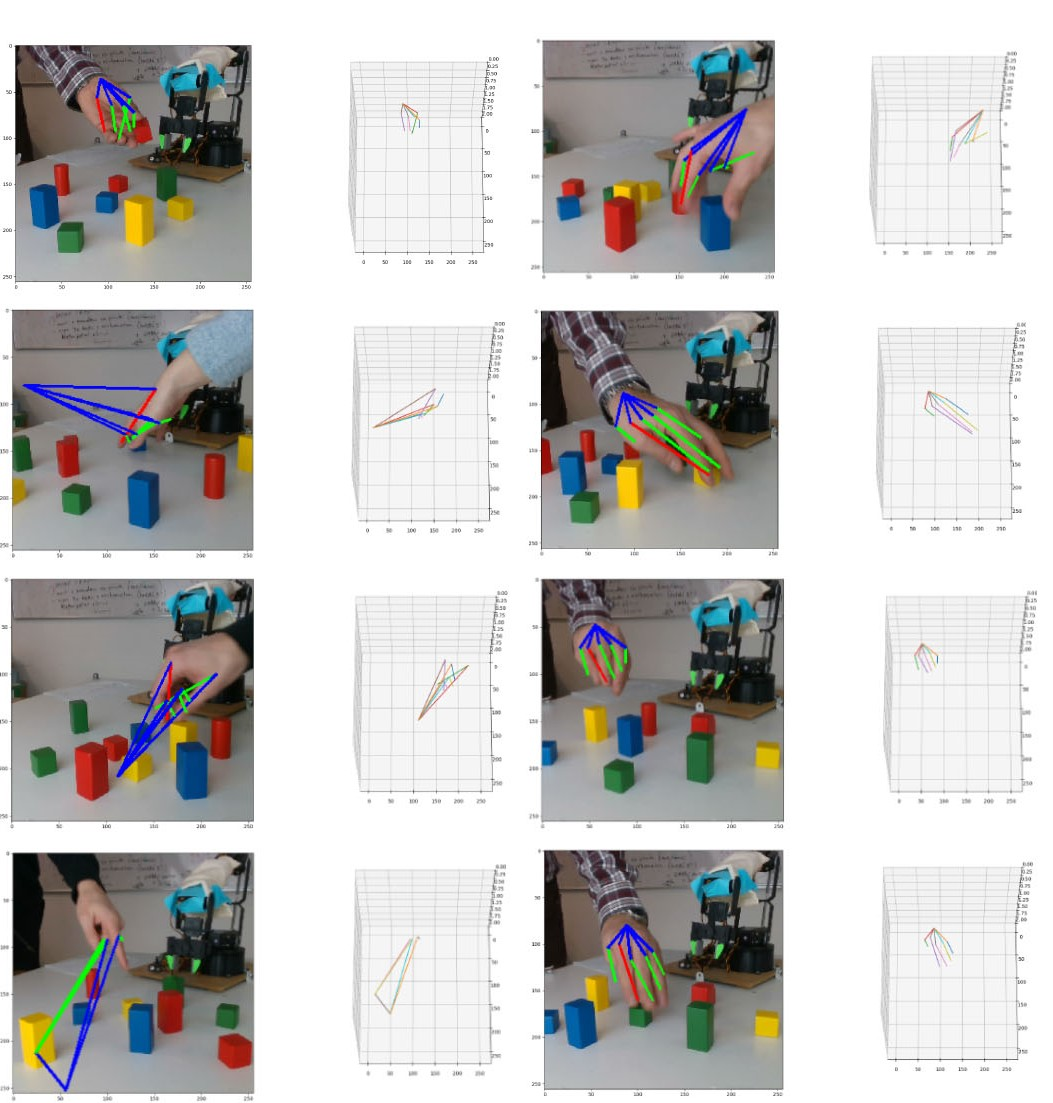
\includegraphics[width=\textwidth]{images/predicted_hands.jpg}
		\caption{Príklady obrázkov s predikovanými súradnicami. Ukazovák je zvýraznený červenou úsečkou, ostatné prsty zelenou a spojenia prstov so zápästím sú označené modrou úsečkou.}
		\label{img:predicted_hands}
	\end{center}
\end{figure}